\chapter{Patrones de Diseño}

\section{Definición}
\paragraph*{\textcolor{blue}{aquí la definición de patrones de diseño <<Los patrones de diseño con cosas que sirven para diseñar sofware>>}}
\subsection{Patrones de diseño de estructura}
\paragraph*{\textcolor{blue}{definición de patrones de estructurales}}
\subsection{Patrones de diseño de creación}
\paragraph*{\textcolor{blue}{definición de patrones creacionales}}
\subsection{Patrones de diseño de comportamiento}
\paragraph*{\textcolor{blue}{definición de patrones ``comportamientales''}}


\section{Objeto de acceso a datos}\label{sec-dao}

El patrón Objeto de Acceso a Datos (DAO por sus siglas en inglés) es definido por Gupta\cite{OCPJavaSE7} como la abstracción y encapsulación de todo el acceso a la fuente de datos (bases de datos, archivos de texto plano, etc.). Maneja la conexión con la fuente de datos para las operaciones de lectura y escritura, previene al usuario de conocer cómo se hacen la lectura y escritura mientras que le permite al usuario especificar que datos obtener o escribir.
El ocasiones el patrón DAO se presenta acompaño de algún patrón de creación para liberar al usuario de la necesidad de conocer la forma de crear el objeto DAO\cite{OCPJavaSE7}\cite{OCAPJavaSE7}.\\
El patrón DAO comúnmente ofrece las siguientes:
\begin{enumerate}
	\item [] \textbf{buscar}: Realiza la búsqueda de un único elemento, en caso de no encontrarse tal elemento la respuesta es nula.
	\item [] \textbf{listar}: Extrae todos los elementos, el resultado puede utilizar estrategias de paginación.
	\item [] \textbf{insertar}: Guarda un nuevo elemento en la fuente de datos.
	\item [] \textbf{actualizar}: Actualiza la información de un elemento existente en la fuente de datos.
	\item [] \textbf{borrar}: Borra el registro de un elemento en la fuente de datos.
\end{enumerate}


\section{Modelo-Vista-Controlador}\label{sec-mvc}
Para Sarcar\cite{JavaDesignPatternsExamples} el patrón Modelo Vista Controlador (MVC) es un patrón de arquitectura que consiste de tres grandes componentes: Modelo, Vista y Controlador. El Controlador conduce la comunicación entre la Vista y el Modelo, en la Figura \ref{fig:dia-mvc-simple} se muestra el flujo de comunicación entre los componentes MVC.
\begin{enumerate}
	\item \textbf{Modelo}: tiene la responsabilidad de manejar el acceso a los datos persistentes y la lógica de negocio, usualmente se acompaña del patrón DAO\footnote{Ver sección \ref{sec-dao}} para el manejo de datos.
	\item \textbf{Vista}: es la capa de presentación, es responsable de mostrar los datos al actor\footnote{Puede ser una persona u otro sistema} que use el sistema.
	\item \textbf{Controlador}: es el intermediario entre la Vista y el Modelo: comunica las peticiones de la vista al modelo y los datos del modelo a la vista.
\end{enumerate}
\begin{figure}[h]
  \centering
  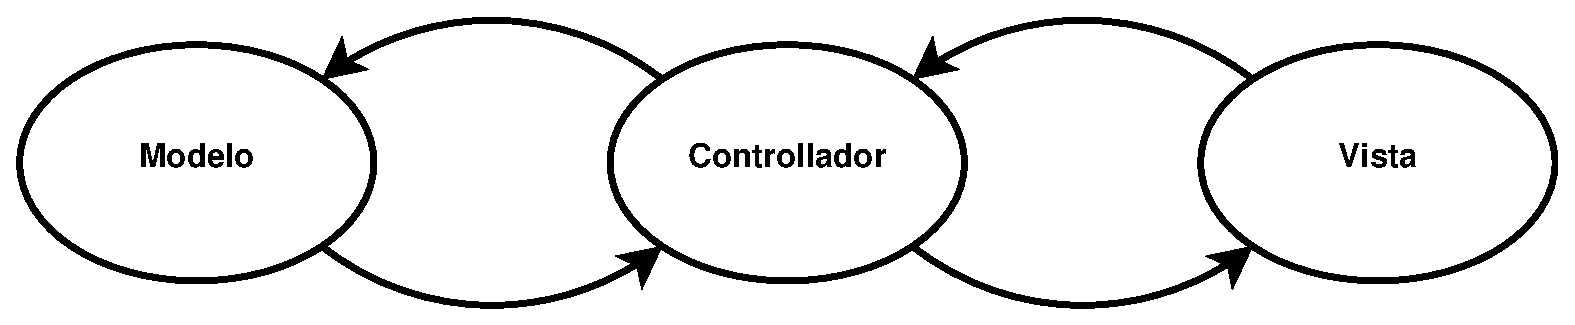
\includegraphics[scale=0.4]{dia-mvc-simple}
  \caption{Diagrama del patrón MVC.}
  \label{fig:dia-mvc-simple}
\end{figure}
